\chapter{Results}
\label{ch:results}

In this chapter, the results from each task are presented and discussed. The results include plots of the HRIR, HRTF frequency response, IIR filter coefficients, and the combined model's impulse response. 

\section{Task 1: HRIR Model}
\label{sec:results_task1}

As seen in \autoref{fig:hrir_multiple}, the Head-Related Impulse Response (HRIR) varies with the angle of incidence. The figure shows the impulse responses for both the left and right ears at angles of \(-30^\circ\), \(0^\circ\), and \(90^\circ\). The figure has an artificial offset between the different angles to be able to visualize all angles clearly since multiple angles can share the same sample delay.

\begin{figure}[H]
    \centering
    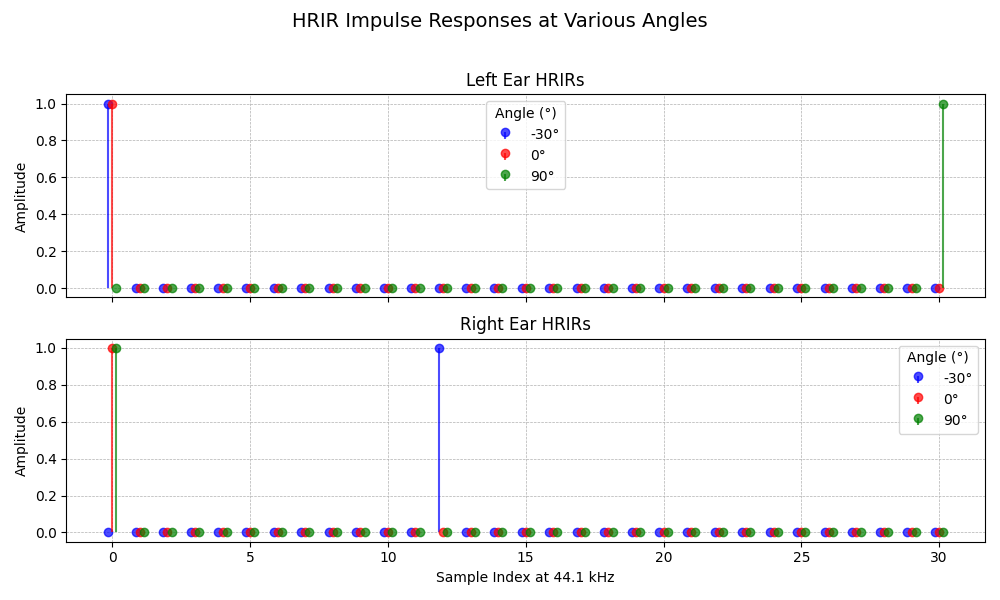
\includegraphics[width=0.9\textwidth]{data/figures/task_1/hrir_impulse_responses_multiple_angles.png}
    \caption{Head-Related Impulse Response (HRIR) for multiple angles of incidence.}
    \label{fig:hrir_multiple}
\end{figure}

For the angle of \(-30^\circ\), the left ear receives the impulse first, followed by the right ear after a short delay, illustrating the interaural time difference. While at \(0^\circ\), both ears receive the impulse simultaneously, indicating no time difference. At \(90^\circ\), the right ear receives the impulse first, with a more significant delay before the left ear's impulse, demonstrating a larger interaural time difference.

\section{Task 2: HRTF Frequency Response}
\label{sec:results_task2}

The Head-Related Transfer Function (HRTF) frequency responses for multiple angles of incidence are shown in \autoref{fig:hrtf_multiple}. This figure illustrates how the frequency response varies with the angle of incidence for both the left and right ears. 

\begin{figure}[H]
    \centering
    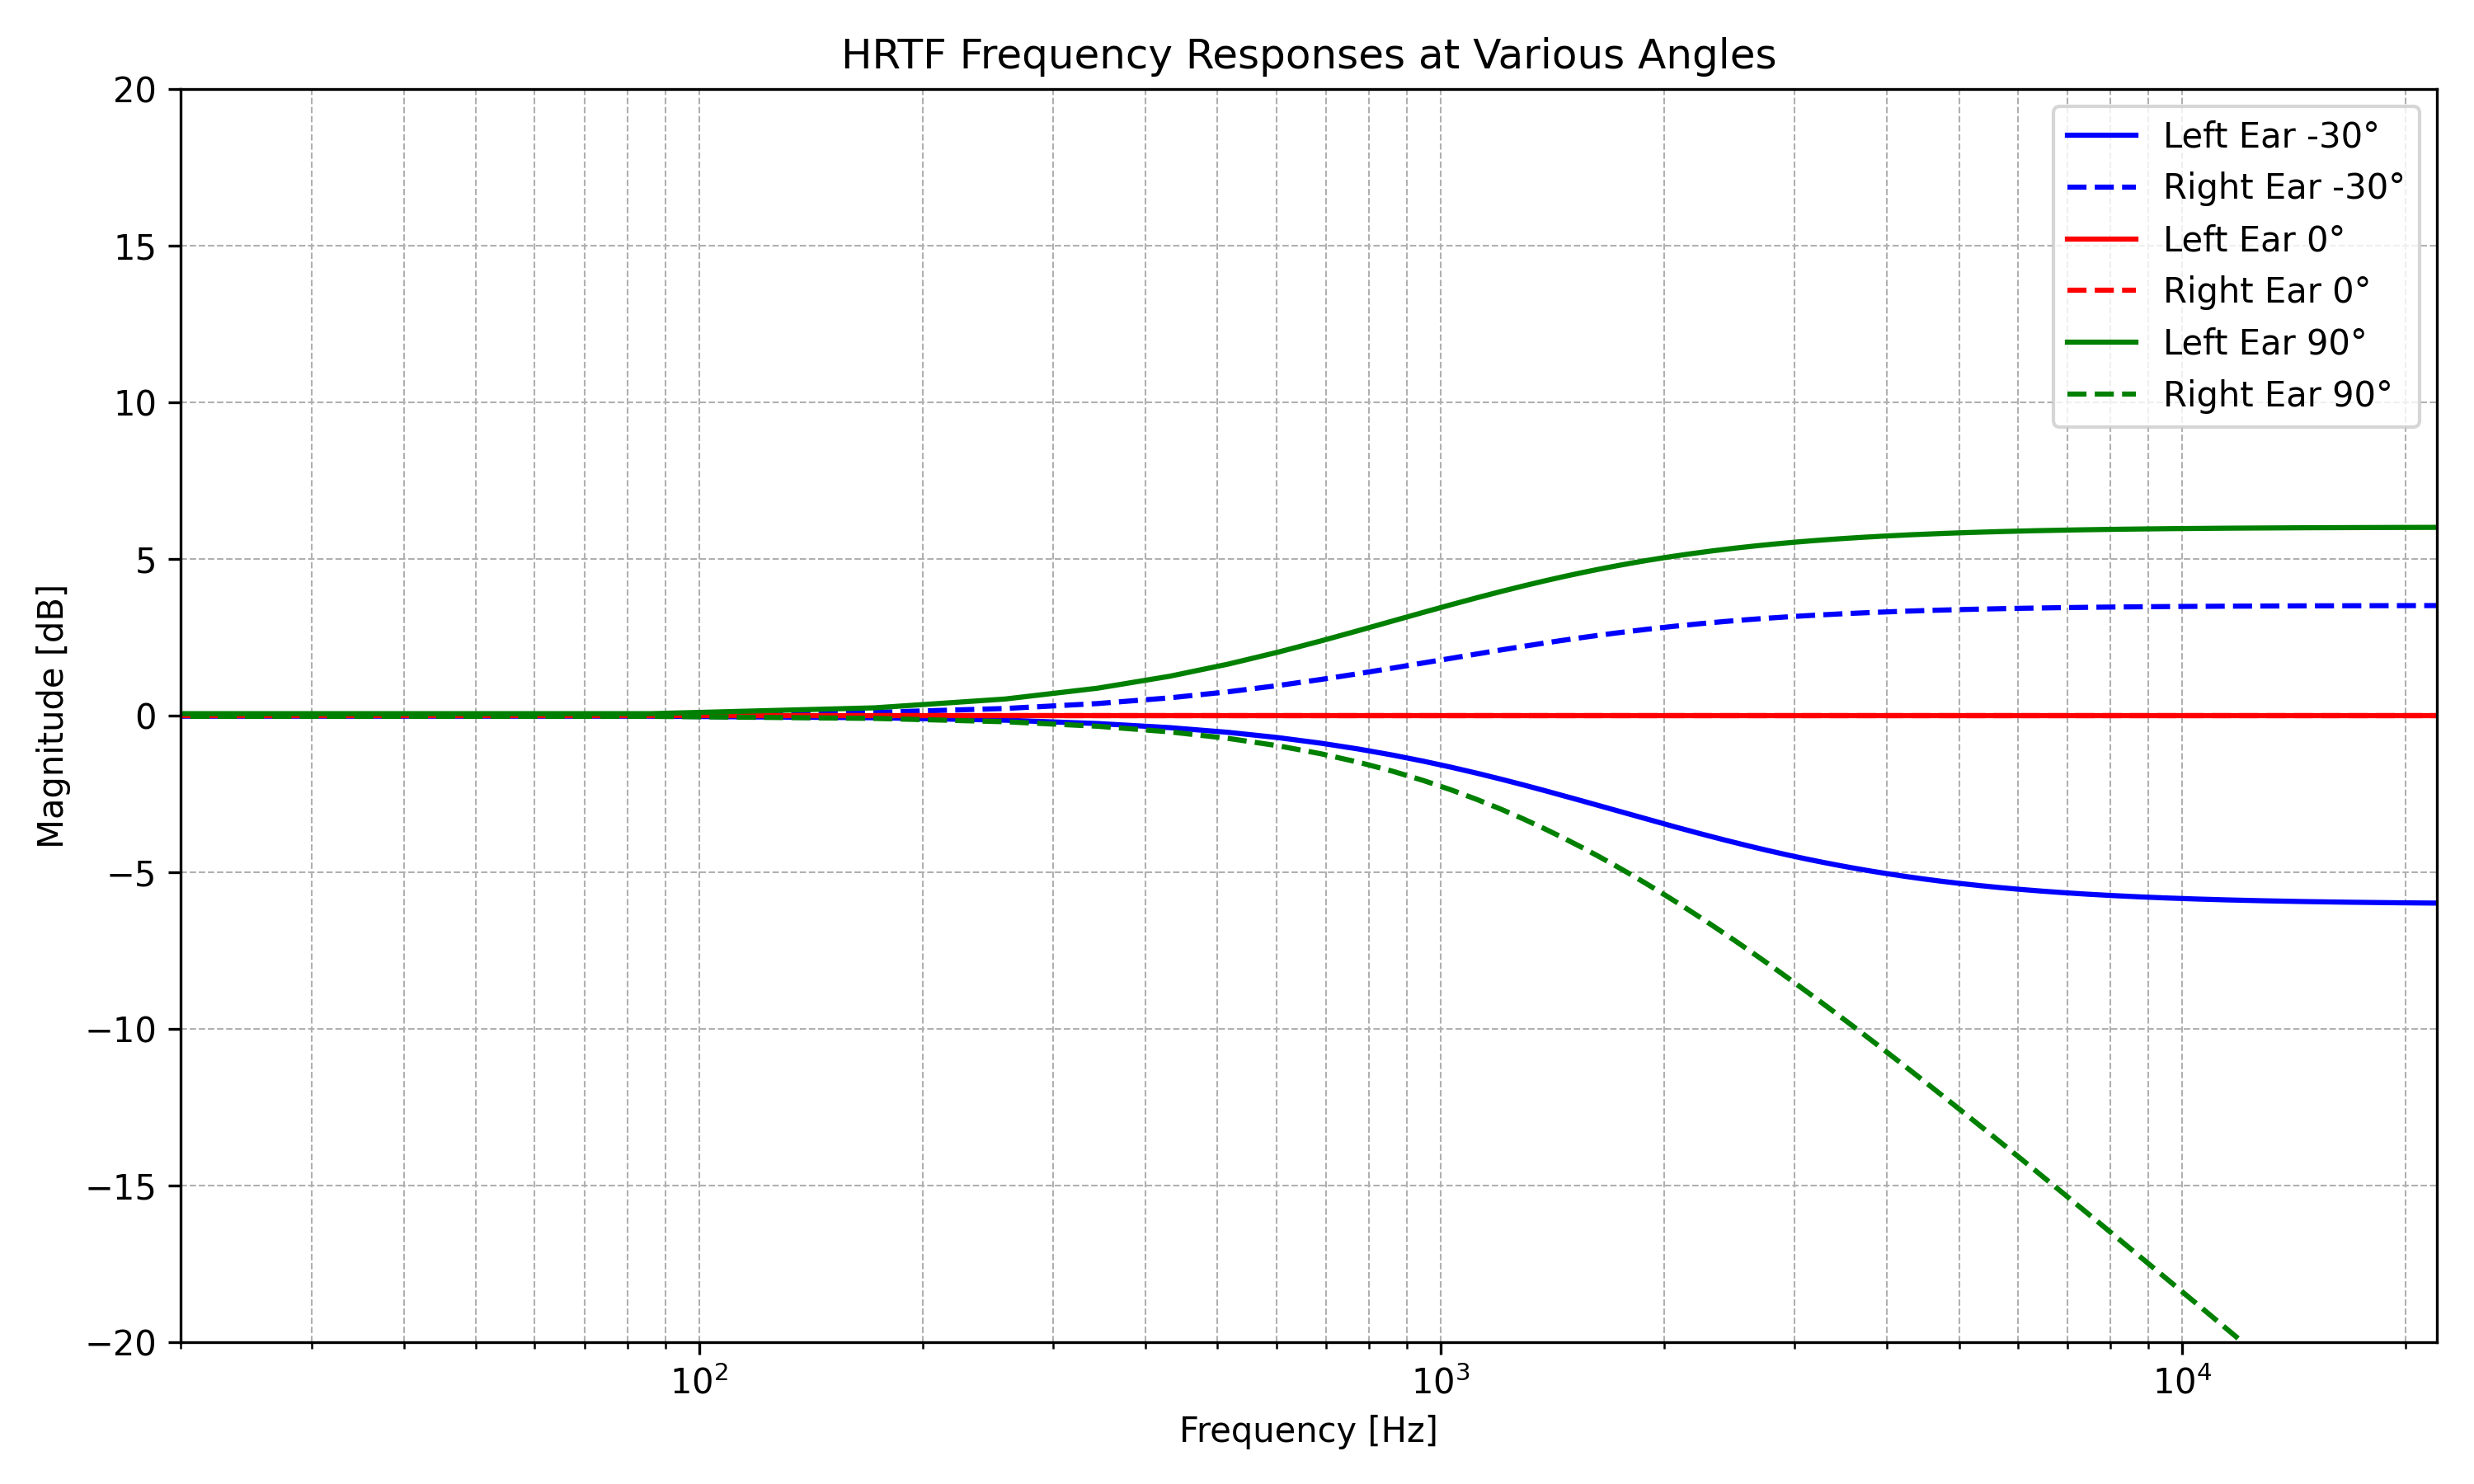
\includegraphics[width=0.9\textwidth]{data/figures/task_2/hrtf_frequency_responses_multiple_angles.png}
    \caption{Head-Related Transfer Function (HRTF) frequency responses for multiple angles of incidence.}
    \label{fig:hrtf_multiple}
\end{figure}

The frequency responses exhibit distinct characteristics depending on the angle, demonstrating the directional filtering effect of the head. For instance, at \(-30^\circ\), the left ear shows a boost in frequencies higher than 2 kHz compared to the right ear, which is attenuated for these frequencies. At \(0^\circ\), both ears have similar frequency responses, indicating a sound from a source directly in front.

The sharper the angle (closer to $\pm 90^\circ$), the more pronounced the differences in frequency response between the two ears as the frequency increases. 

\section{Task 3: HRTF IIR Filter}
\label{sec:results_task3}

The IIR filter coefficients derived from the bilinear transform for the HRTF model are presented in \autoref{tab:hrtfiir_coefficients}. The table lists the coefficients \( B_0 \), \( B_1 \), and \( A_1 \) for both the left and right ears. These coefficients are essential for implementing the IIR filter that approximates the HRTF in the discrete-time domain.

\begin{table}[H]
    \centering
    \caption{IIR filter coefficients for the Head-Related Transfer Function (HRTF) model, derived using the bilinear transform.}
    \label{tab:hrtfiir_coefficients}
    \begin{tabular}{lccccc}
        \toprule
        \textbf{Angle (°)} & \textbf{A$_1$} & \textbf{B$_{0,L}$} & \textbf{B$_{0,R}$} & \textbf{B$_{1,L}$} & \textbf{B$_{1,R}$} \\
        \midrule
        -90 & -0.8409 & 1.0000 & 1.9205 & 0.0795 & -1.7614 \\
        -60 & -0.8409 & 1.0617 & 1.8588 & -0.0438 & -1.6380 \\
        -30 & -0.8409 & 1.2301 & 1.6903 & -0.3807 & -1.3011 \\
         0  & -0.8409 & 1.4602 & 1.4602 & -0.8409 & -0.8409 \\
         30 & -0.8409 & 1.6903 & 1.2301 & -1.3011 & -0.3807 \\
         60 & -0.8409 & 1.8588 & 1.0617 & -1.6380 & -0.0438 \\
         90 & -0.8409 & 1.9205 & 1.0000 & -1.7614 & 0.0795 \\
        \bottomrule
    \end{tabular}
\end{table}

As observed, the feedforward coefficients \( B_0 \) and \( B_1 \) vary significantly with the angle of incidence, while the pole coefficient \( A_1 \) remains constant across angles.

These coefficients can be used to implement the IIR filter in a digital signal processing system to simulate the HRTF effect for different sound source directions, shown in \autoref{fig:hrtfiir_filter}.

\begin{figure}[H]
    \centering
    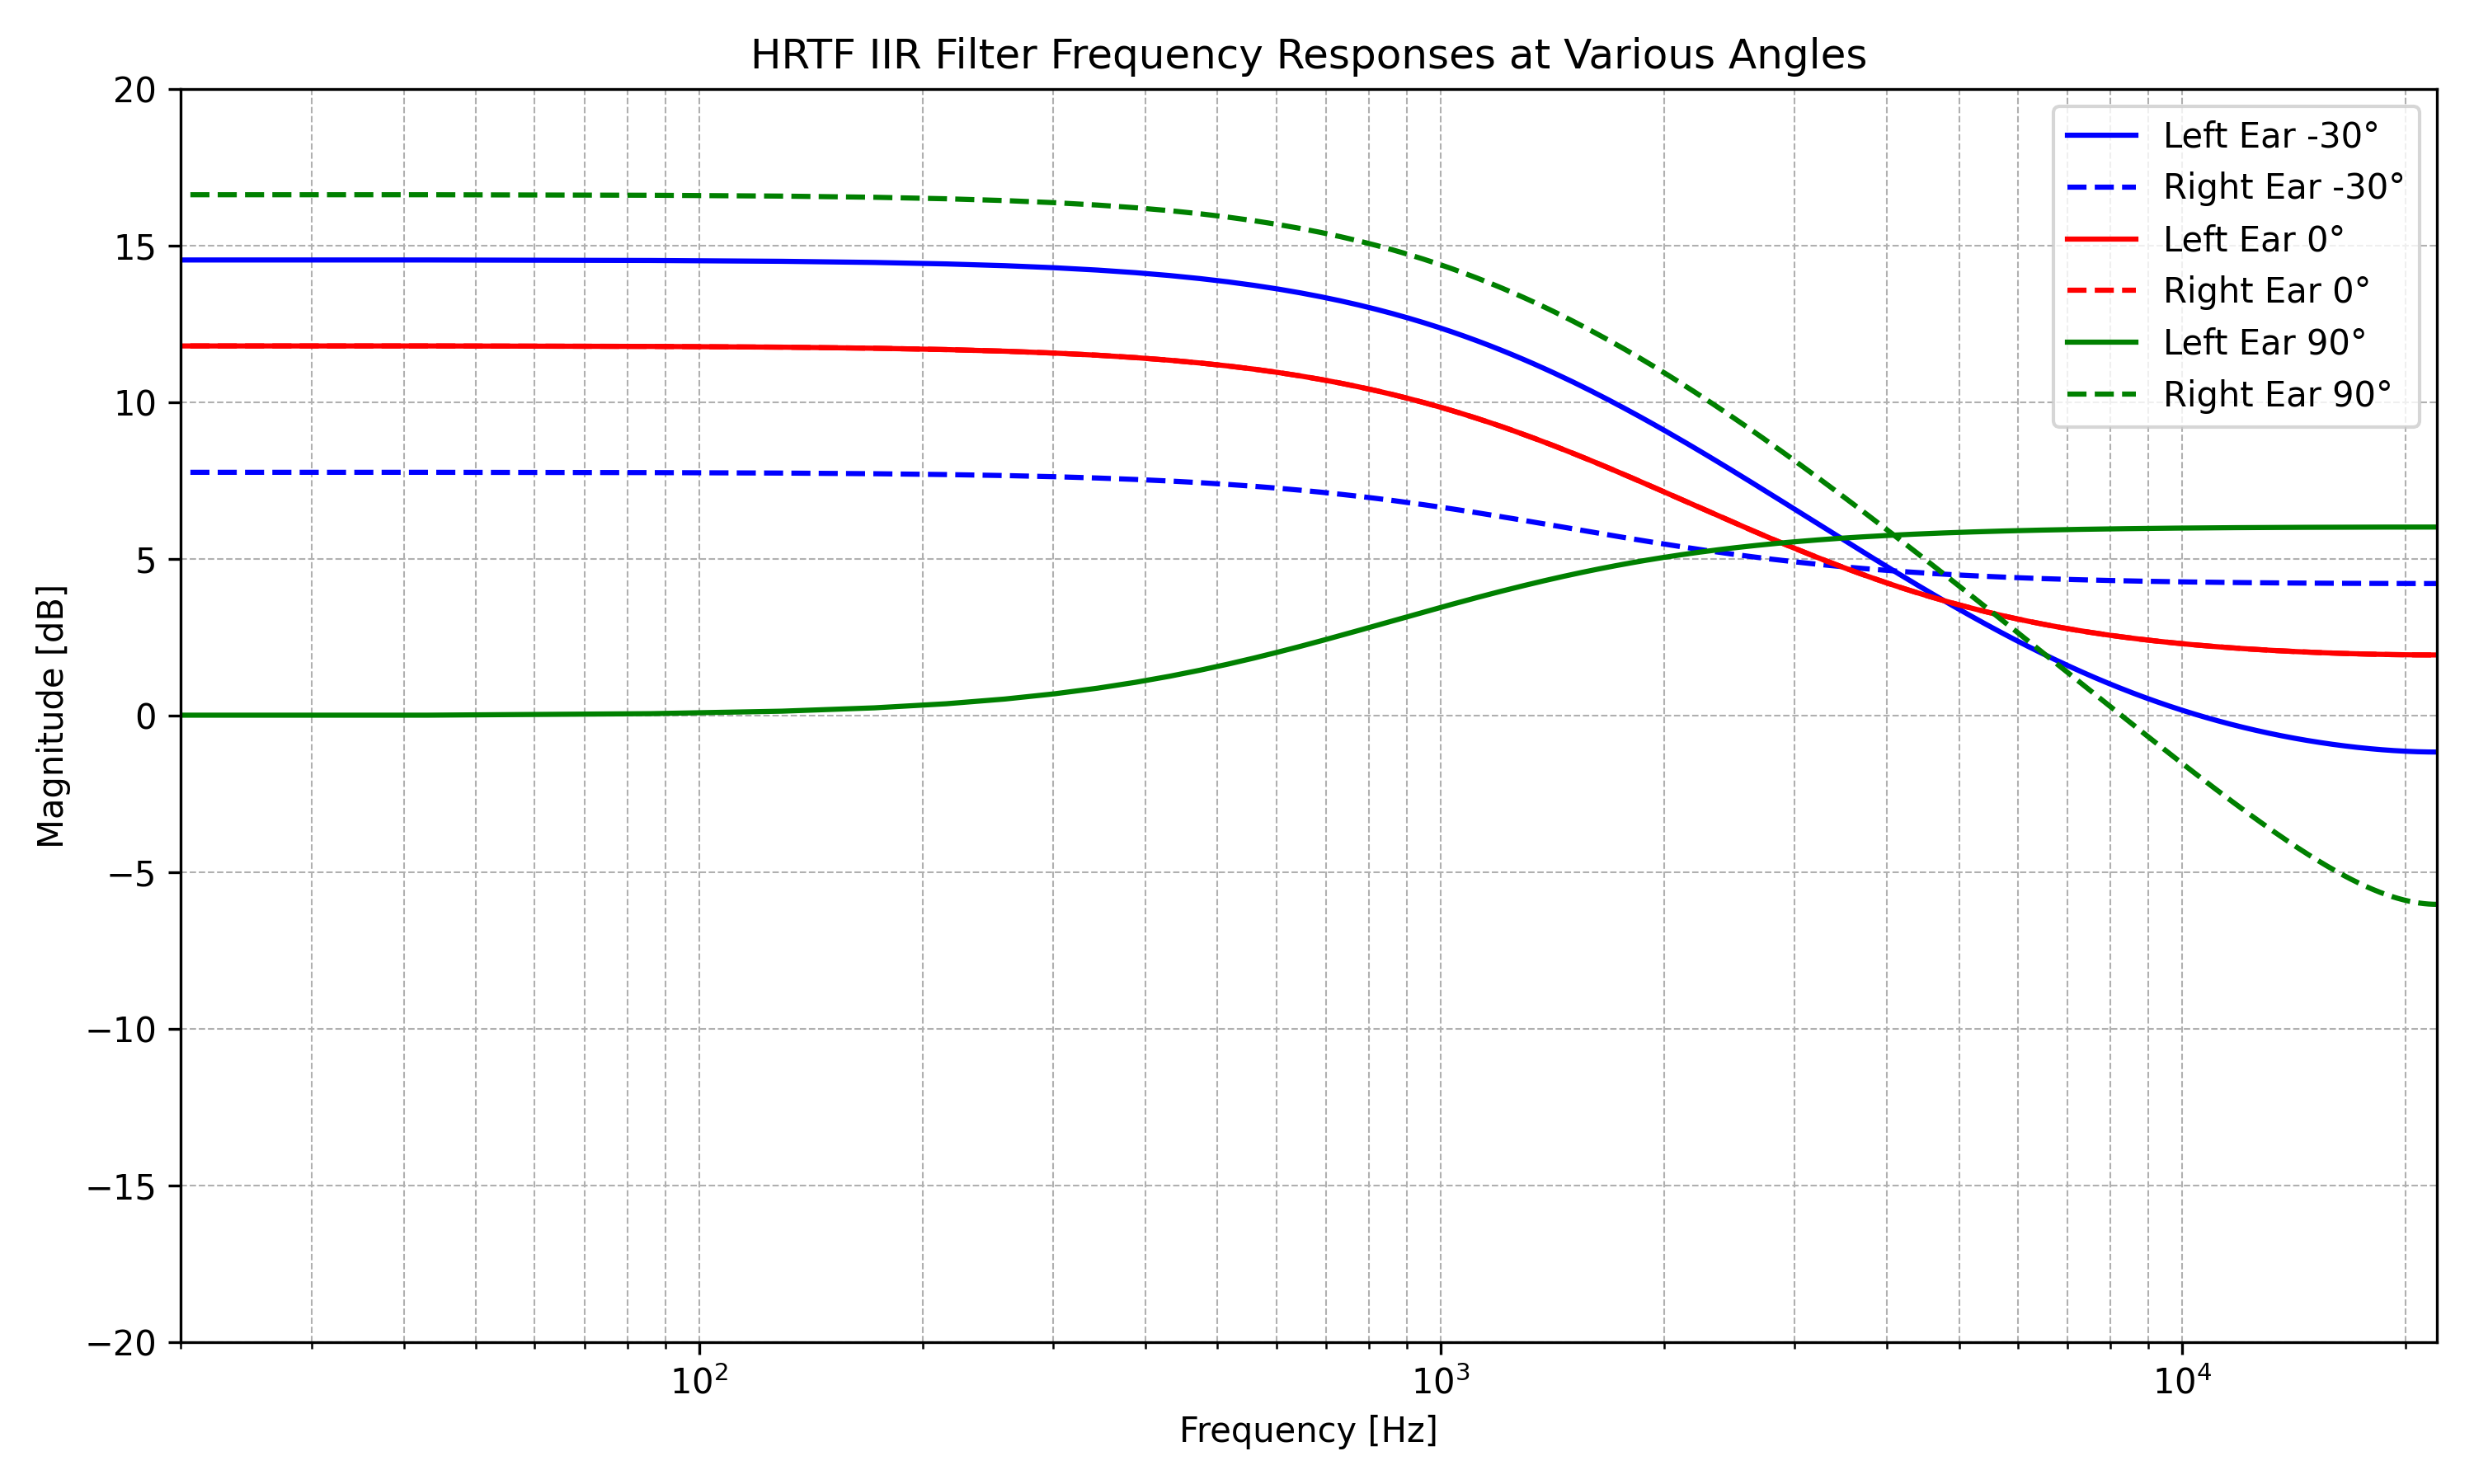
\includegraphics[width=0.9\textwidth]{data/figures/task_3/hrtfiir_freq_responses_multiple_angles.png}
    \caption{IIR filter frequency responses for the Head-Related Transfer Function (HRTF) model at multiple angles of incidence.}
    \label{fig:hrtfiir_filter}
\end{figure}

\section{Task 4: Combined Model}
\label{sec:results_task4}

The combined Head-Related Impulse Response (HRIR) model, which integrates the interaural time difference (ITD) with the HRTF IIR filter, is illustrated in \autoref{fig:combined_hrir_time}.

\begin{figure}[H]
    \centering
    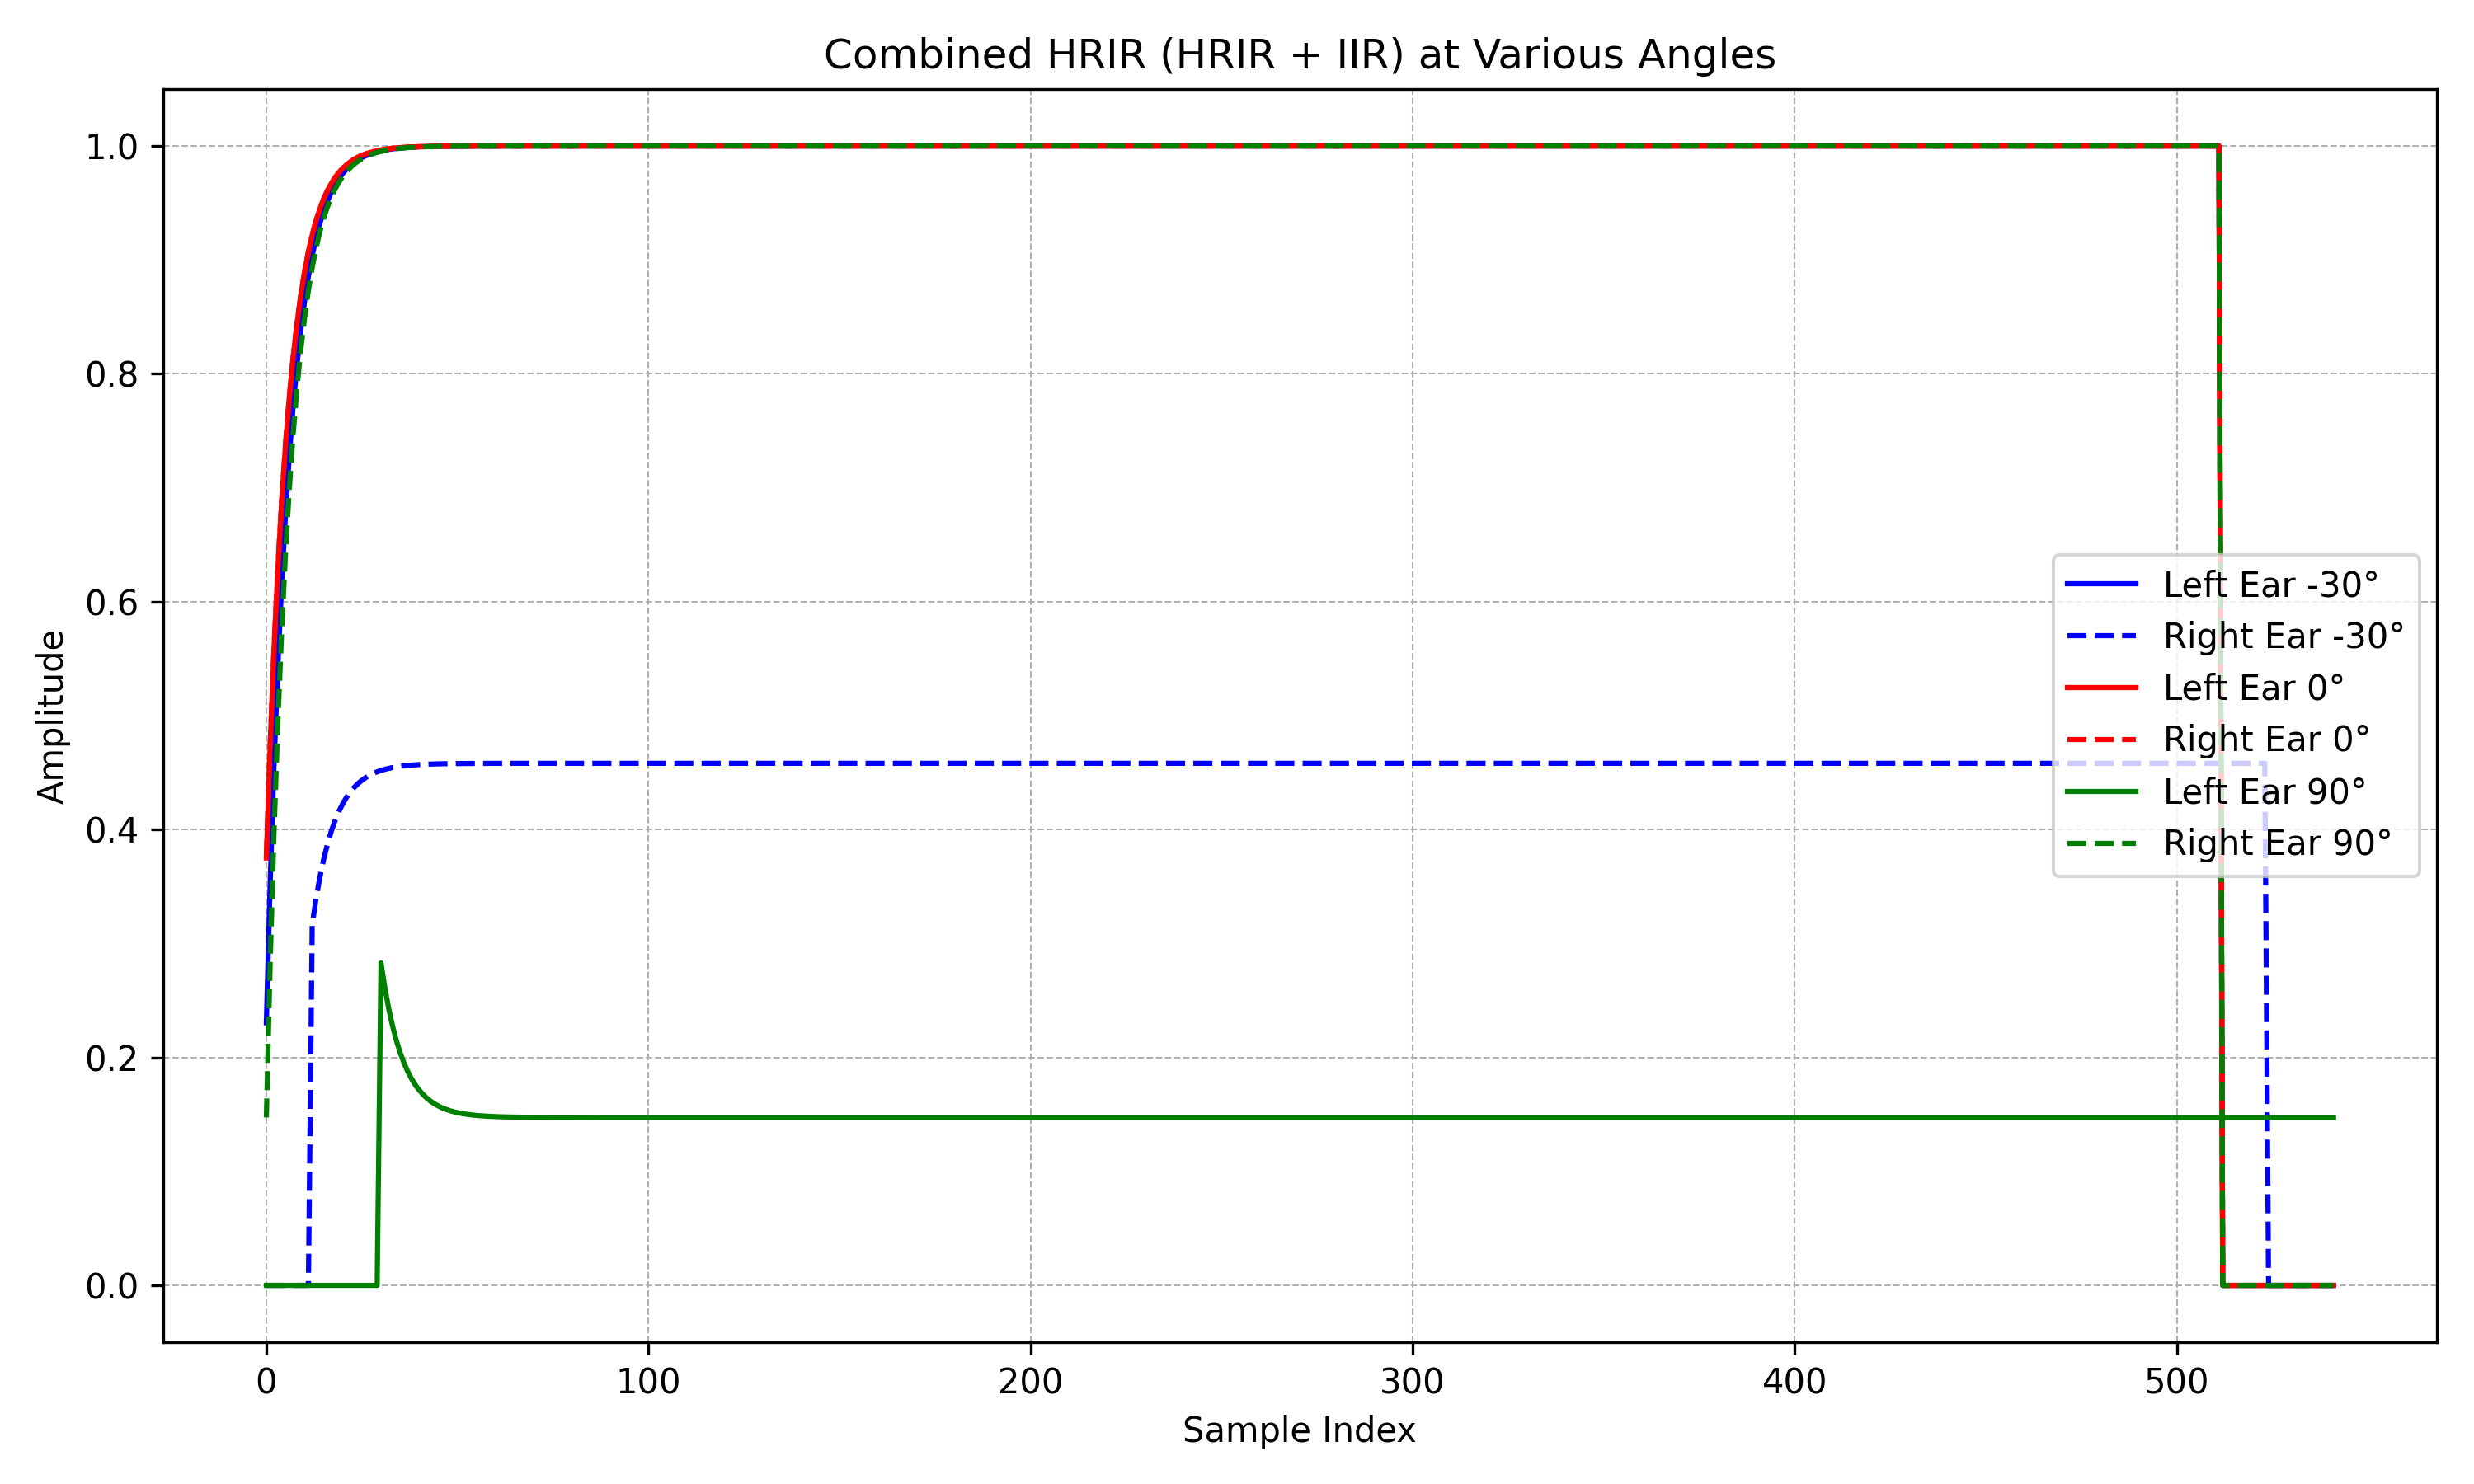
\includegraphics[width=0.9\textwidth]{data/figures/task_4/combined_hrir_time_multiple.png}
    \caption{Impulse responses of the combined HRIR model for multiple angles of incidence.}
    \label{fig:combined_hrir_time}
\end{figure}

This figure shows the time-domain impulse responses for the specified angles. For the angle of \(-30^\circ\), the left ear receives the impulse first, followed by a weakened response in the right ear after a delay, consistent with the ITD.

For angles closer to \(0^\circ\), both ears receive impulses nearly simultaneously, with similar amplitude responses. At \(90^\circ\), the right ear receives the impulse first, with a more attenuated response in the left ear after a longer delay.


\section{Task 5: Sound Demonstration}
\label{sec:results_task5}

As seen in \autoref{fig:sound_demo_waveform}, the waveform of the processed pink noise shows variations in amplitude due to the different angles of incidence. Each angle segment is separated by a brief silence and the changes in amplitude can be observed as the angle changes from \(-90^\circ\) to \(90^\circ\). The left ear shows a decrease in amplitude as the angle moves from \(-90^\circ\) to \(90^\circ\), while the right ear shows an increase.

\begin{figure}[H]
    \centering
    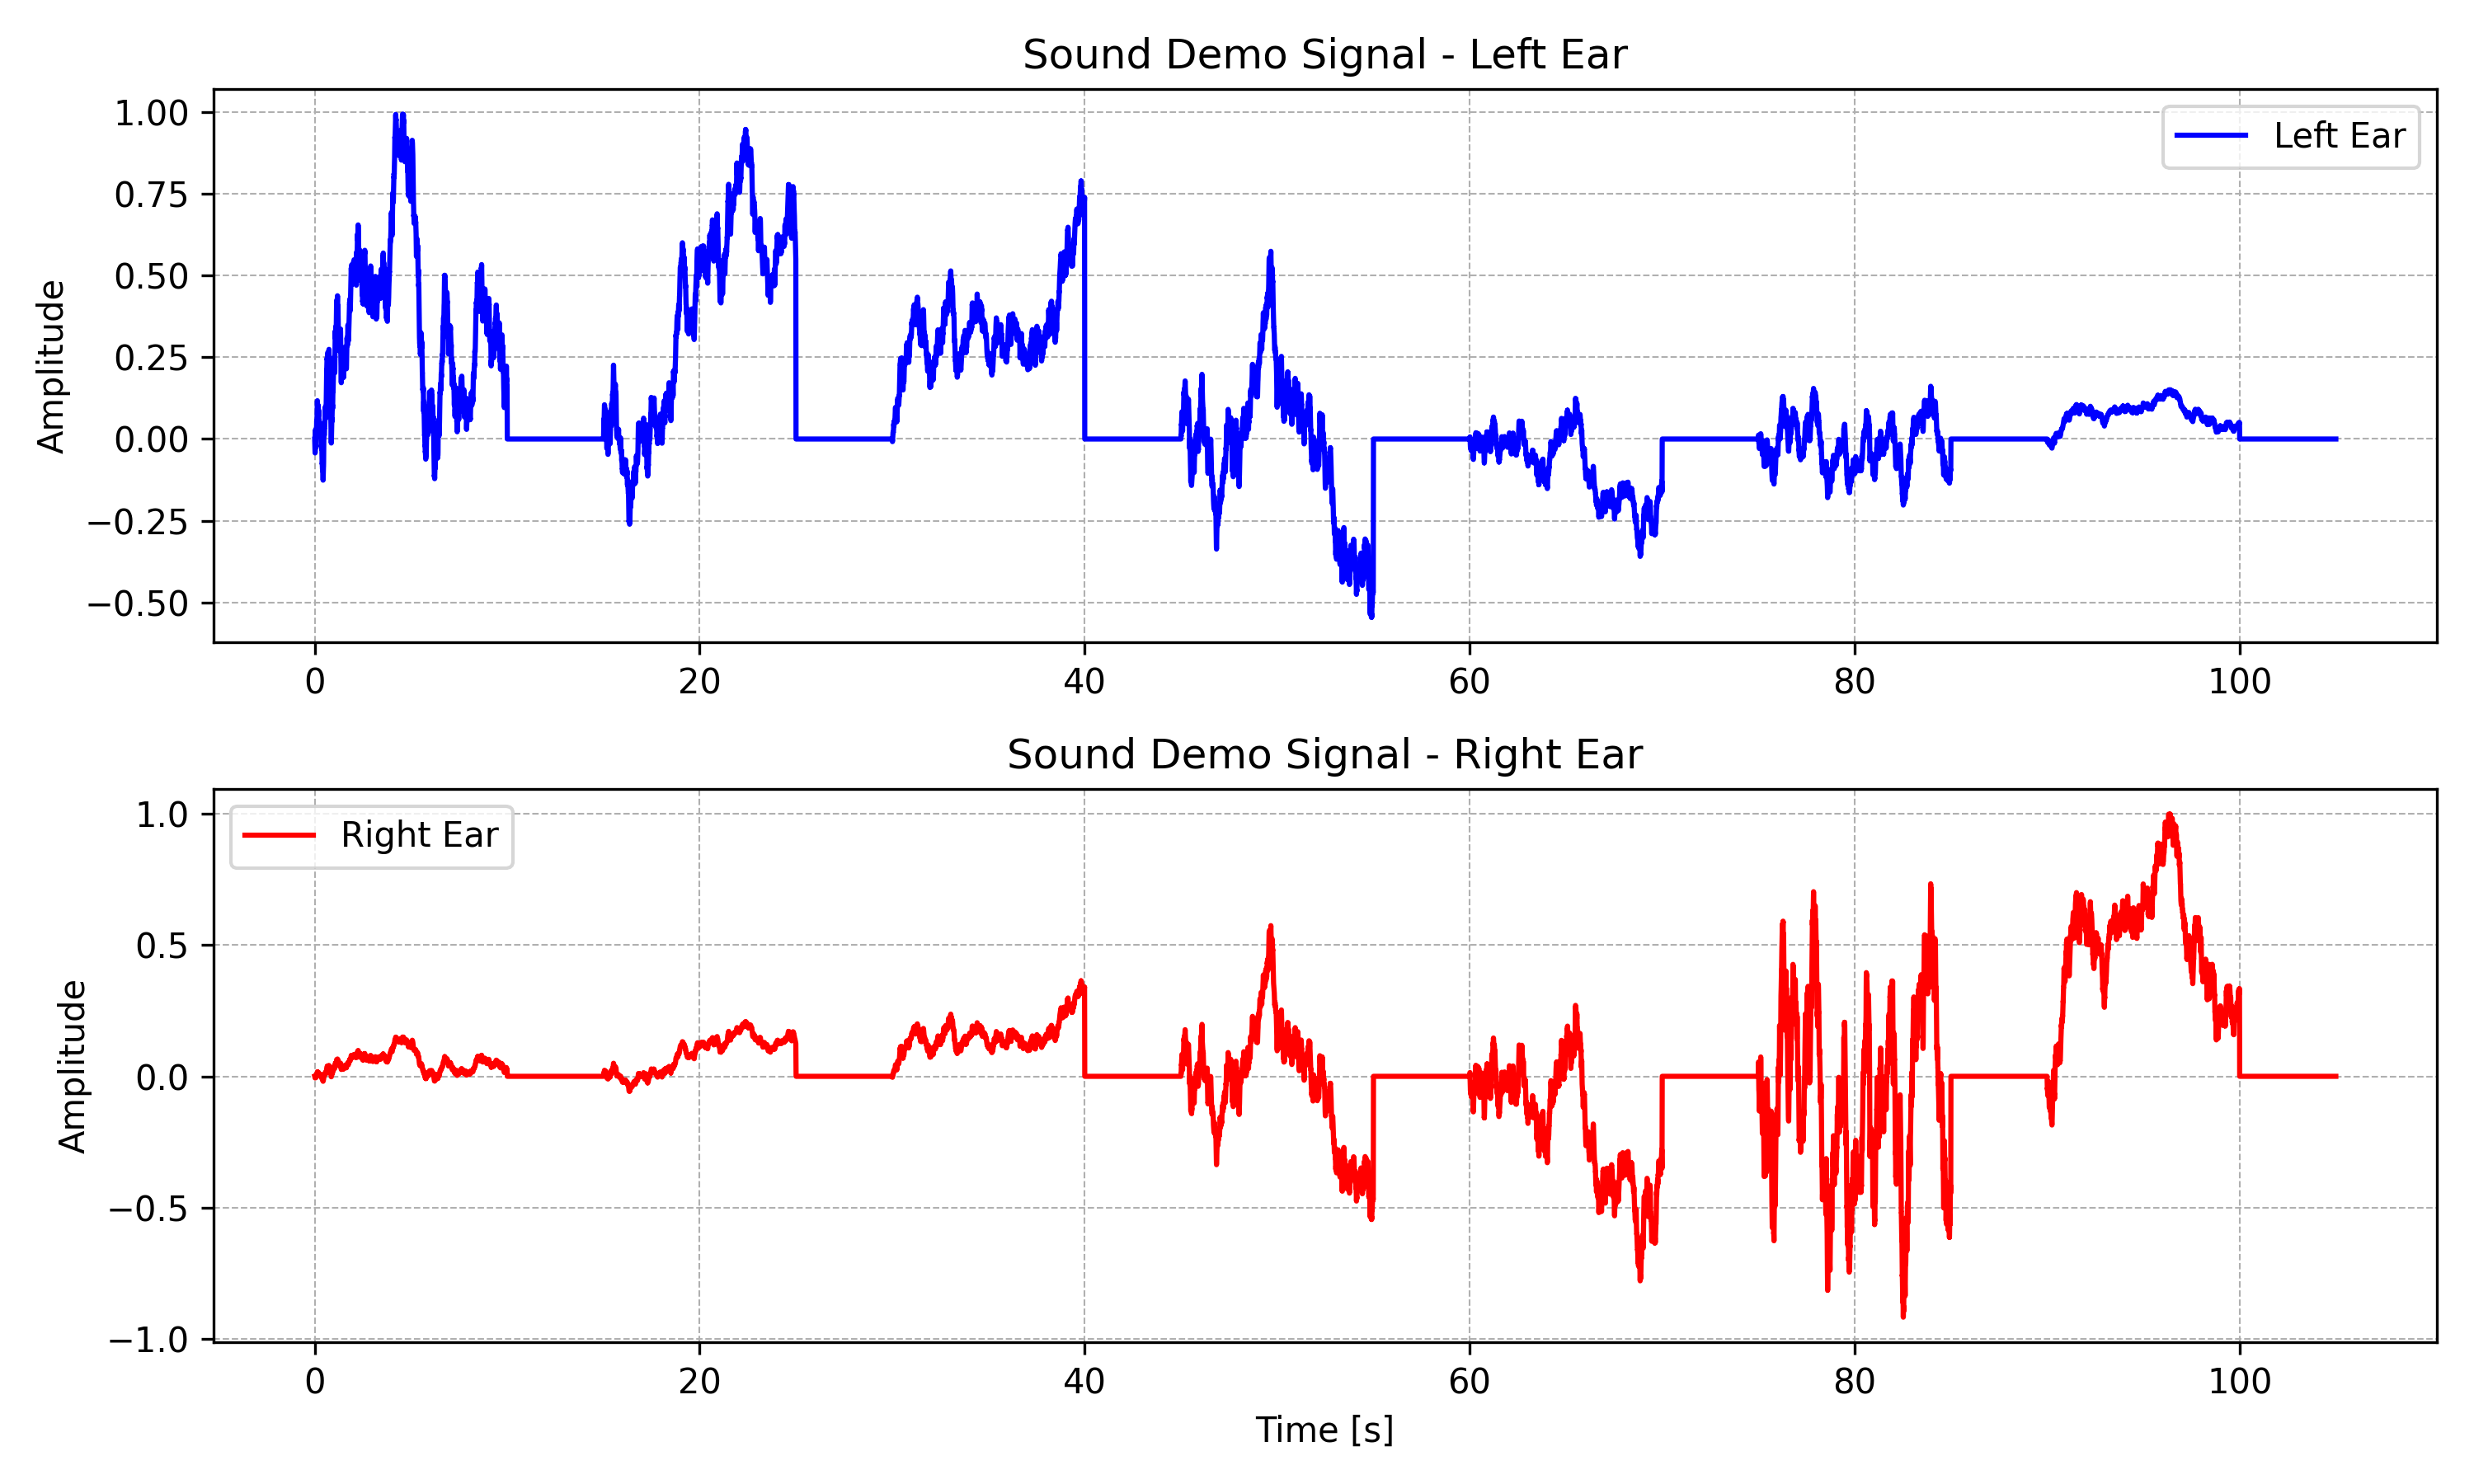
\includegraphics[width=0.9\textwidth]{data/figures/task_5/sound_demo_signal.png}
    \caption{Waveform of the pink noise sound demonstration processed with the combined HRIR and HRTF IIR model for angles from \(-90^\circ\) to \(90^\circ\).}
    \label{fig:sound_demo_waveform}
\end{figure}

